\documentclass[12pt]{article}
\usepackage{graphicx}
\usepackage{psfrag}
\usepackage{epsfig}
\usepackage{subfigure}
\usepackage{amssymb,amsmath}
\usepackage{verbatim}

%\usepackage{doublespace}

\textheight 23cm \topmargin -1cm \leftmargin 0cm

\marginparwidth 0mm    % Largeur des notes marge de droite
\textwidth 16.5cm      % Largeur du texte
\hsize \textwidth      % Longueur d'une ligne
\advance \hsize by -\marginparwidth
\oddsidemargin -4mm    % Marge gauche pages de droite - 1 inch (2.54 cm)
\evensidemargin \oddsidemargin % Idem pour les pages de gauche

\advance\hoffset by 5mm % Pour corriger un decalage residuel sur la gauche

\renewcommand{\hat}{\widehat}
\newcommand{\R}{\mathrm{I\!R\!}}
\newcommand{\C}{\mathrm{I\!\!\!C\!}}
\newcommand{\sinc}{\mbox{sinc}}
\newcommand{\diag}{\mbox{diag}}
\newcommand{\Tr}{\mbox{Tr}}

% commands
\newtheorem{theo}{Theorem}
\newtheorem{proposition}{Proposition}
\newcommand{\nc}{\newcommand}
\nc{\RR}{\mbox{\rm I$\!$R}} \nc{\dsp}{\displaystyle}
\nc{\Div}{\mbox{\rm div }} \nc{\beequ}{\begin{equation}}
\nc{\barr}{\begin{array}} \nc{\earr}{\end{array}}
\nc{\eequ}{\end{equation}} \nc{\BFF}{\hbox{\boldmath{${\cal
F}$}}^{(j)}({\bf y}^s,t)}

\nc{\hr}{\widehat{r}} \nc{\hh}{\widehat{h}} \nc{\hs}{\widehat{s}}
\nc{\hn}{\widehat{n}} \nc{\hw}{\widehat{w}} \nc{\hd}{\widehat{d}}
\nc{\hG}{\widehat{\Gamma}} \nc{\om}{\omega} \nc{\yy}{{\bf y}}
\nc{\ys}{{\bf y}^s} \nc{\yo}{{\bf y}_0} \nc{\xp}{{\bf x}_p}
\nc{\xr}{{\bf x}_r} \nc{\co}{{\cal O}}
\renewcommand\labelenumi{\alph{enumi})}
\begin{document}
\begin{center}
\textbf{Practice Set 4 Solutions}
\end{center}
\paragraph{Problem 1} The transmit covariances for the various cases are given as follows.
\begin{enumerate}
\item When the transmitter has no knowledge of the channel, use $\pmb \Sigma=\frac{P}{2}I$
\item With no phase information, it is impossible to correctly aim a beam towards the receiver. Thus it is best to transmit equal power to all spatial directions. Mathematically, the power transmitted to angle $\theta$ is given by 
$\mathrm{E}\{ \lvert \mathbf a^H(\theta) \mathbf s \rvert ^2 \} $, and should be independent of $\theta$. Here, $\mathbf a^H(\theta)$ is the array steering vector and is of the form $[1, e^{j 2\pi \Delta \sin(\theta) / \lambda}]^T$ for a two-element array. 

Let $$\mathbf R_{\mathbf {ss}} = \begin{bmatrix} a & b \\ b^\ast & c \end{bmatrix} $$ be the transmit covariance matrix. Then,
\begin{eqnarray*}
	\mathrm{E}\{ \lvert \mathbf a^H(\theta) \mathbf s \rvert ^2 \} 
		&=& \mathbf a(\theta)^H \mathbf R_{\mathbf {ss}}\mathbf a(\theta) \\
		&=& a + c + 2 \mathop{\mathrm{Re}}(b e^{j 2\pi \Delta \sin(\theta) / \lambda}) 
\end{eqnarray*}
If follows that $b=0$ and thus $\mathbf{R_{ss}}$ is a diagonal matrix. Plugging into the capacity formula, we obtain 
\begin{eqnarray*}
	C &=& \log \left( 1 + \frac{E_s}{N_0 M_T}  [h_1, h_2] \begin{bmatrix} a & 0 \\ 0 & c\end{bmatrix} \begin{bmatrix} h_1^\ast \\ h_2^\ast \end{bmatrix} \right) \\
	&=& \log \left( 1 + \frac{E_s}{N_0 M_T}  \left( \lvert h_1\rvert^2 a +  \lvert h_2 \lvert^2 b \right) \right),
\end{eqnarray*}
which we should maximize subject to $\mathrm{trace}(\mathbf{R_{ss}}) = a+c \leq M_T$. Clearly, $C$ is maximized by
\begin{eqnarray*}
	\mathbf{R_{ss}} &=& \begin{cases}
	                    	\begin{bmatrix} M_T & 0 \\ 0 & 0 \end{bmatrix} & \text{if $\lvert h_1\rvert \geq \lvert h_2\rvert$}, \\[5mm]
	                    	\begin{bmatrix} 0 & 0 \\ 0 & M_T \end{bmatrix} & \text{if $\lvert h_1\rvert < \lvert h_2\rvert$}. \\
	                    \end{cases}
\end{eqnarray*}
The transmit covariance matrix $\pmb \Sigma$ is then given as 
\begin{eqnarray*}
	\pmb \Sigma &=& \begin{cases}
	                    	\begin{bmatrix} P & 0 \\ 0 & 0 \end{bmatrix} & \text{if $\lvert h_1\rvert \geq \lvert h_2\rvert$}, \\[5mm]
	                    	\begin{bmatrix} 0 & 0 \\ 0 & P \end{bmatrix} & \text{if $\lvert h_1\rvert < \lvert h_2\rvert$}. \\
	                    \end{cases}
\end{eqnarray*}


\item When the transmitter has full knowledge of the channel, use MRC at the transmitter. This can also be shown using the SVD.
\begin{equation*}
\pmb \Sigma=
\frac{P}{2(|h_1|^2+|h_2|^2)}
\left[ \begin{array}{cc}
|h_1|^2 & h_1^*h_2\\
h_2^*h_1 & |h_2|^2\\
\end{array}\right ]
\end{equation*}
\end{enumerate}


\paragraph{Problem 2} \begin{enumerate}
\item Fig. \ref{fig:p3_corr} plots the capacity versus SNR for
different receive correlation values.  Here, we use equation (4.39) in the book with
\[
{\bf R}_t={\bf I} \text{ and }{\bf R}_r=\left[\begin{array}{cc} 1
& \rho\\ \rho^* & 1\end{array}\right].
\]
The capacity for the case with no correlation ($\rho=0$) and the
case with $\rho=0.2$ have almost identical capacities.  Use
equation (4.40) in the book to see why the two capacities are so
similar (the high SNR difference is only about 0.06 bps/Hz). Only
higher values for correlation seem to affect the ergodic capacity.
The Matlab script follows:
\begin{footnotesize}
\verbatiminput{p3.m}
\end{footnotesize}

\item Fig. \ref{fig:p3_kfac} plots the capacity vs SNR for various
$K$-factors.  As $K$-factor increases the capacity at high SNR
values decreases.  I used the following script:
\begin{footnotesize}
\verbatiminput{p3_2.m}
\end{footnotesize}

\begin{figure}
  % Requires \usepackage{graphicx}
  \centering
  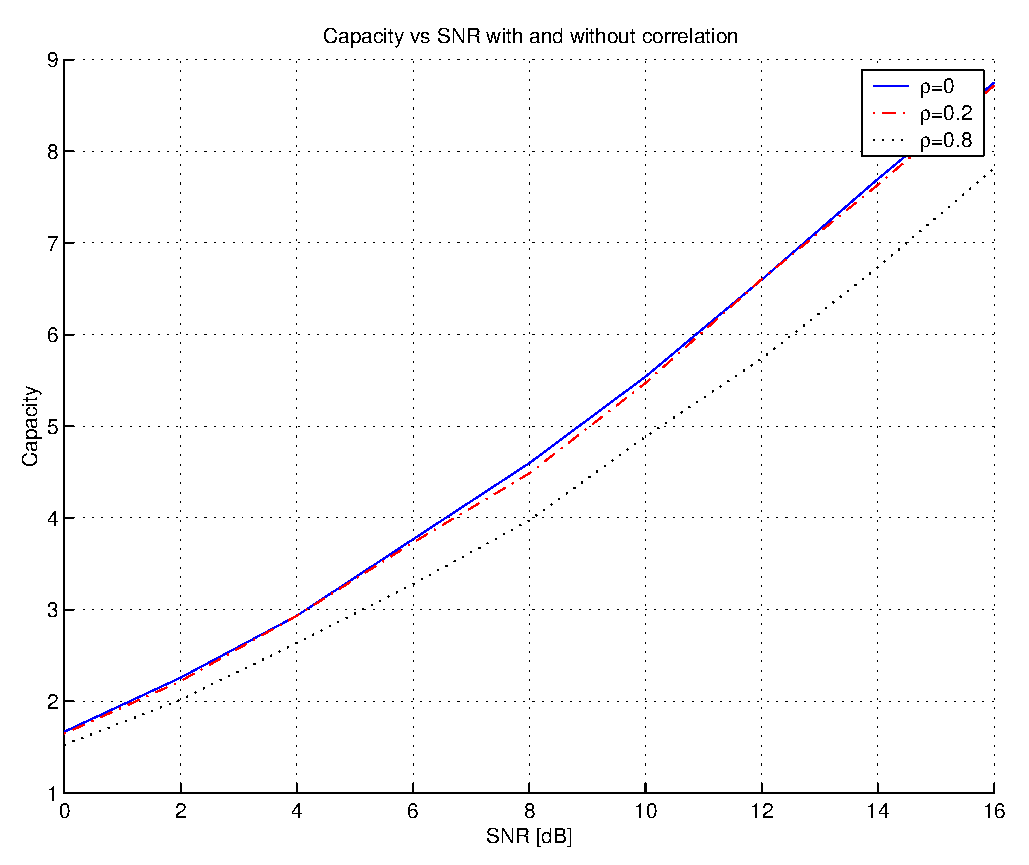
\includegraphics[width=4in]{p3_correlation.eps}\\
  \caption{\footnotesize Capacity vs SNR with and without correlation.}
  \label{fig:p3_corr}
\end{figure}
\begin{figure}
  % Requires \usepackage{graphicx}
  \centering
  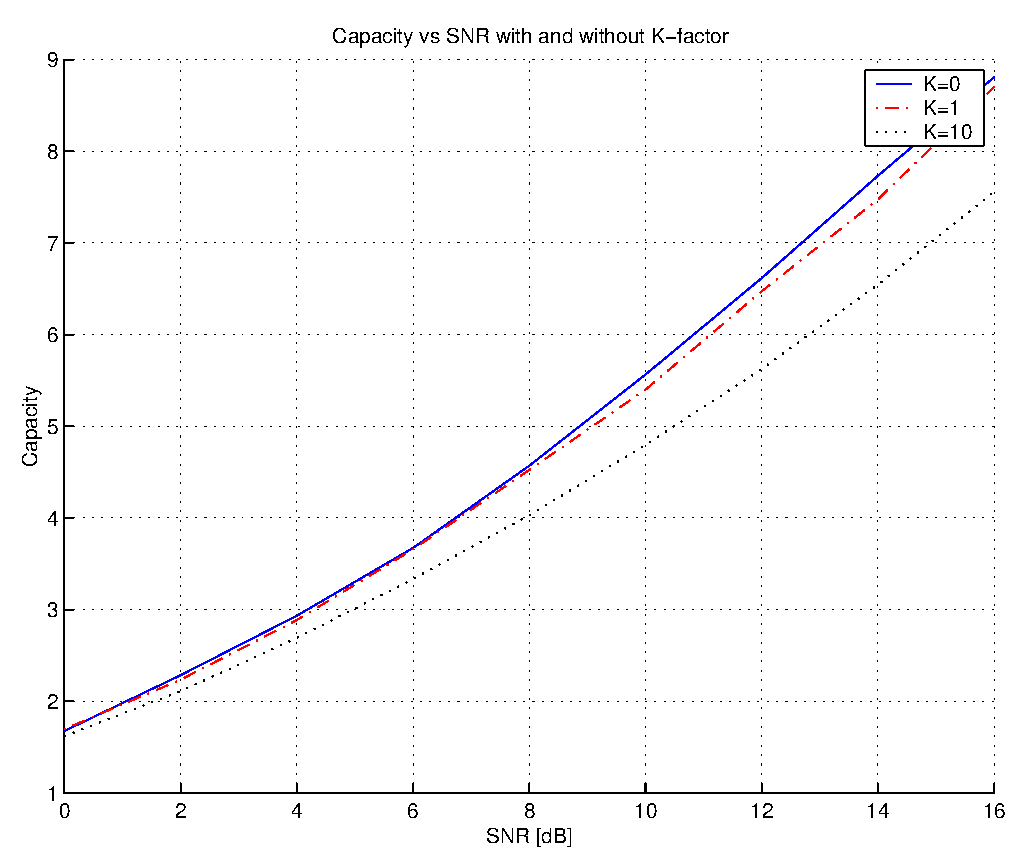
\includegraphics[width=4in]{p3_kfactor.eps}\\
  \caption{\footnotesize Capacity vs SNR with and without $K$-factor.}
  \label{fig:p3_kfac}
\end{figure}
\end{enumerate}


\paragraph{Problem 3} {\it Alamouti Code and Channel Estimation Errors}\\
\begin{enumerate}
\item With Alamouti coding, the received signals can be expressed as
\begin{equation*}
\begin{split}
\left[ \begin{array}{c}
y_1 \\
y_2^*
\end{array}
\right] &= \sqrt{\frac{E_s}{2}} \left[
\begin{array}{cc}
h_1+\epsilon_1 & h_2+\epsilon_2 \\
h_2^*+\epsilon_2^* & -h_1^*-\epsilon_1^*
\end{array}
\right] \left[
\begin{array}{c} s_1 \\ s_2 \end{array}
\right] + \left[ \begin{array}{c} n_1 \\n_2^* \end{array}
\right]\\
{\bf y} &= \sqrt{\frac{E_s}{2}}{\bf Hs}+{\bf n}
\end{split}
\end{equation*}
With a channel estimate ${\bf \hat H}$, Alamouti decoding becomes
\begin{equation*}
{\bf \hat y} = \sqrt{\frac{E_s}{2}}{\bf \hat H}^H {\bf H} + {\bf
\hat H}^H {\bf n},
\end{equation*}
where the channel estimate is
\begin{equation*}
{\bf \hat H} = \left[ \begin{array}{cc} h_1 & h_2\\
 h_2^* & -h_1^*
\end{array} \right].
\end{equation*}
On decoding we have \begin{equation*}
\begin{split}
{\bf \hat H}{\bf H} &  = \left[ \begin{array}{cc} h_1 & h_2\\
h_2^* & -h_1^*\end{array} \right]^H\left[
\begin{array}{cc}
h_1+\epsilon_1 & h_2+\epsilon_2 \\
h_2^*+\epsilon_2^* & -h_1^*-\epsilon_1^*
\end{array}
\right]\\
& = \left[
\begin{array}{cc}
|h_1|^2 + h_1^* \epsilon_1 + |h_2|^2 + h_2\epsilon_2^* & h_1^*\epsilon_2-h_2\epsilon_1^* \\
h_2^*\epsilon_1-h_1\epsilon_2^* & |h_1|^2  + h_1\epsilon_1^* + |h_2|^2 + h_2^*\epsilon_2
\end{array}
\right] \\
& = \left[
\begin{array}{cc}
|h_1|^2  + |h_2|^2  & 0 \\
0 & |h_1|^2  + |h_2|^2
\end{array}
\right]+ \left[
\begin{array}{cc}
h_1^* \epsilon_1 + h_2\epsilon_2^* & h_1^*\epsilon_2-h_2\epsilon_1^* \\
h_2^*\epsilon_1-h_1\epsilon_2^* &  h_1\epsilon_1^* + h_2^*\epsilon_2
\end{array}
\right]
\end{split}
\end{equation*}
Therefore our decoded signal ${\bf \hat y}$ becomes
\begin{equation*}
\begin{split}
{\bf \hat y} & =\sqrt{\frac{E_s}{2}} \left[
\begin{array}{cc}
|h_1|^2  + |h_2|^2  & 0 \\
0 & |h_1|^2  + |h_2|^2
\end{array}
\right] {\bf s} + \sqrt{\frac{E_s}{2}}\left[
\begin{array}{cc}
h_1^* \epsilon_1 + h_2\epsilon_2^* & h_1^*\epsilon_2-h_2\epsilon_1^* \\
h_2^*\epsilon_1-h_1\epsilon_2^* &  h_1\epsilon_1^* + h_2^*\epsilon_2
\end{array}
\right] {\bf s} + {\bf \hat H}^H {\bf n}
\\
& = {\bf \tilde y}_{signal} + {\bf \tilde y}_{mismatch} + {\bf \tilde
n}_{noise}
\end{split}
\end{equation*}

\item The main diagonal terms represent the noise due to channel
estimation errors from the symbol itself. The off-diagonal terms
represent inter-symbol interference generated by the channel
estimation errors.

\item We assume that $\epsilon_i$ and $s_i$ are independent.
\begin{equation*}
\begin{split}
{\bf y}_{signal,1} & =  \sqrt{\frac{E_s}{2}}(|h_1|^2 + |h_2|^2)s_1 \Rightarrow (|h_1|^2 + |h_2|^2)^2 \frac{E_s}{2} \\
{\bf y}_{mismatch,1} & = \sqrt{\frac{E_s}{2}}(h_1^* \epsilon_1 +
h_2 \epsilon_2^*)s_1 + \sqrt{\frac{E_s}{2}}( h_1^* \epsilon_2 -
h_2 \epsilon_1^*) s_2 \Rightarrow 2(
|h_1|^2 \sigma_e^2 + |h_2|^2 \sigma_e^2 ) \frac{E_s}{2} \\
{\bf y}_{noise} & = h_1n_1 + h_2n_2
\\
& = \left(|h_1|^2+|h_2|^2 \right) \sigma_n^2 = ( |h_1|^2 +|h_2|^2) \sigma_n^2
\end{split}
\end{equation*}
The effective SNR becomes
\begin{equation*}
SNR_{AC} = \frac{(|h_1|^2 + |h_2|^2)^2 E_s/2}{(|h_1|^2 +
|h_2|^2)(\sigma_n^2 + 2 \sigma_e^2 E_s/2)} = \frac{ \frac{1}{2} \rho \lVert \mathbf h \rVert^2}{ 1 + \rho \sigma_e^2 }
\end{equation*}
\item AC is sensitive to channel estimation errors.
\begin{figure} [hhh]
\vspace{3mm}
\centerline{\psfig{figure=ac_est_error2.eps,width=12cm}}
\caption{ {AC performance with estimation errors.}} \label{fig:ac_est}
\end{figure}
\verbatiminput{ps5p4.m}
\end{enumerate}


\paragraph{Problem 4} {\it Spatial Multiplexing} \\
Recall that we are using zero-forcing receivers. Let $\rho = E_s /  \sigma^2$.
\begin{enumerate}
\item (Horizontal encoding with successive cancellation) Decoding the  first stream with treating the second stream as noise yields the equivalent SINR
$$
	\eta_1 = \frac{ \rho} {M_T} \cdot \frac{1}{[(\mathbf H^H \mathbf H)^{-1}]_{1,1}} \approx 0.1285 \rho
$$
Thus the mutual information for this stream is
$$
	I_1^\text{HE} \approx  \log_2(1+ 0.1285 \rho )
$$
After cancelation of the first stream, the second stream experiences only thermal noise. With $\mathbf h_2$ being the second column of $\mathbf H$, we have
$$
	\eta_2 = \frac{ \rho} {M_T} \lVert \mathbf h_2 \rVert^2 \approx 1.125 \rho
$$
Thus the mutual information for this stream is
$$
	I_2^\text{HE} \approx  \log_2(1+ 1.125 \rho )
$$
 
\item (Diagonal encoding) Recall the encoding structure
$$
\left[ \begin{array}{ccc}
S_{11} & S_{21} & 0\\
0 & S_{12} & S_{22}
\end{array} \right ]
$$
When $S_{11}$ is decoded, only thermal noise will play a role. Thus
$$
	\eta_{11} =  \frac{ \rho} {M_T} \lVert \mathbf h_1 \rVert^2 \approx 0.5312 \rho
$$ 
where $\mathbf h_1$ is the first column of $\mathbf H$.
For $S_{12}$, the component $S_{21}$ will act as interference, leading to 
$$
	\eta_{12} = \frac{ \rho} {M_T} \cdot \frac{1}{[(\mathbf H^H \mathbf H)^{-1}]_{2,2}} \approx 0.2721 \rho
$$
Next, for $S_{21}$, perfect cancelation applies and only thermal noise remains,
$$
	\eta_{21} =  \frac{ \rho} {M_T} \lVert \mathbf h_1 \rVert^2 \approx 0.5312 \rho
$$ 
Finally, $S_{22}$ does not experience interference by construction. Thus
$$
	\eta_{22} =  \frac{ \rho} {M_T} \lVert \mathbf h_2 \rVert^2 \approx 1.125 \rho
$$
where again, $\mathbf h_2$ is the second column of $\mathbf H$.
The average mutual information for the two data streams are thus
\begin{eqnarray*}
	I_1^\text{DE} &\approx &  1/2 \, \log_2(1+ 0.5312 \rho ) +1/2 \, \log_2(1+ 0.2721 \rho ) \\
	I_2^\text{DE} &\approx & 1/2 \, \log_2(1+ 0.5312 \rho ) +1/2 \, \log_2(1+ 1.125 \rho ).
\end{eqnarray*}
\paragraph{Problem 5} {\it (Channel correlations) } \quad
Consider a $2\times 2$ MIMO channel
\begin{enumerate}
\item The transmit and receive correlation matrices can be
expressed as follows:
\[
{\bf R}_T=\left[
\begin{array}{cc}
1 & \alpha\\
\alpha^* & 1
\end{array}
\right],\mbox{ and } {\bf R}_R = \left[\begin{array}{cc}
1 & \beta\\
\beta^* & 1
\end{array}
\right]
\]
Then the Kronecker product can be expanded as:
\[
{\bf R}_T^T \otimes {\bf R}_R=\left[
\begin{array}{cccc}
1 & \beta & \alpha^* & \alpha^*\beta\\
\beta^* & 1 & \alpha^*\beta^* & \alpha^*\\
\alpha & \alpha\beta & 1 & \beta\\
\alpha\beta^* & \alpha & \beta^* & 1\\
\end{array}
\right]
\]
Consider a general $4\times 4$ correlation matrix ${\bf
R}=[r_{ij}]$. In order for the relation in question to hold one
must have:
\begin{eqnarray}
r_{14}&=&r_{24}r_{12}\Rightarrow
E[h_{11}h^*_{22}]=E[h_{21}h^*_{22}]E[h_{11}h^*_{21}]\\
r_{23}&=&r_{13}r_{21}\Rightarrow
E[h_{21}h^*_{12}]=E[h_{11}h^*_{12}]E[h_{21}h^*_{11}]
\end{eqnarray}
and
\begin{eqnarray}
r_{13}&=&r_{24}\Rightarrow E[h_{11}h^*_{12}]=E[h_{21}h^*_{22}]\\
r_{12}&=&r_{34}\Rightarrow E[h_{11}h^*_{21}]=E[h_{12}h^*_{22}]
\end{eqnarray}
\item The first set of relation implies that if there is both
transmit and receive correlation, the correlation between channel
elements without any common transmitter and receiver will be
non-zero.  The second set of relations means that in order to
compute the transmit correlation, it doesn't matter which receive
antenna is chosen as the reference.  Additionally, it doesn't matter which transmit antenna is chosen as the reference for computing the receive correlation.  This model assumes that the antennas in each set of transmit antennas interact with the same scatterers.  The same is true for the receive antennas.
\end{enumerate}

\end{enumerate}

\end{document}

















